\chapter{De centrale limietstelling}
\label{ch:centrale-limietstelling}

In dit hoofdstuk wordt de Centrale Limietstelling geïntroduceerd (zie Sectie~\ref{sec:centrale-limietstelling}). Dit is voor het vakgebied van de statistiek een enorm belangrijk resultaat omdat de gehele theorie van statistische toetsen (zie Hoofdstuk~\ref{ch:toetsingsprocedures}) hierop gebaseerd is. De Centrale Limietstelling laat toe om metingen op basis van een steekproef onder bepaalde voorwaarden te veralgemenen naar de populatie als geheel.

We bespreken eveneens het concept van puntschatters en betrouwbaarheidsintervallen. Een puntschatter is een getal dat berekend wordt uit de steekproef, waarmee men een schatting wil maken van een eigenschap van de populatie. Het steekproefgemiddelde $\overline{x}$ is bijvoorbeeld een puntschatter voor het populatiegemiddelde $\mu$. Een betrouwbaarheidsinterval drukt uit tussen welke grenzen men vermoedt dat een bepaalde waarde zich bevindt, en hoe zeker men hiervan is. Een 95\%-betrouwbaarheidsinterval voor het populatiegemiddelde, bijvoorbeeld, is een interval dat als met het experiment genoeg herhaalt, men in 95\% van de gevallen zeker is dat dat interval het populatiegemiddelde bevat.

Voordat we deze begrippen kunnen introduceren, is het nodig eerst enkele begrippen uit de kansrekening te herhalen (zie Sectie~\ref{sec:kansverdeling-steekproef}) en de normale verdeling  (zie Sectie~\ref{sec:normale-verdeling}) te bespreken.

\section{Leerdoelen}
\label{sec:centrale-limietstelling-leerdoelen}

Na dit hoofdstuk moet je in staat zijn om:

\begin{itemize}
  \item De volgende begrippen uit te leggen en toe te passen:
  \begin{itemize}
    \item Uitkomstenruimte (universum), gebeurtenis, kansruimte, kans, discrete/continue kansverdeling
    \item Puntschatter, betrouwbaarheidsinterval
    \item Vrijheidsgraden
  \end{itemize}
  \item De kansverdeling van de normale verdeling met gegeven gemiddelde en standaardafwijking te schetsen (Gauss-curve) en gemiddelde en standaardafwijking erop aan te duiden;
  \item De $z$-score van een waarde in een normaal verdeelde stochastische variabele te berekenen;
  \item De linker- ($P(X<x)$) en rechterstaartkans ($P(X>x)$) of combinaties van beide (bv. $P(x<X<y)$) voor een waarde in een normaal verdeelde stochastische variabele te berekenen, en daarbij waar nodig gebruik te maken van de symmetrieregel en de 100\%-regel;
  \item Van een gegeven stochastische variabele te bepalen in hoeverre ze normaal verdeeld is a.h.v.~de kansdichtheidscurve, QQ-plot, scheefheid of kurtosis;
  \item De centrale limietstelling te formuleren (i.h.b. te weten welke kansverdeling het steekproefgemiddelde volgt) en het belang ervan voor statistische analyse uit te leggen.
  \item Een betrouwbaarheidsinterval voor het populatiegemiddelde van een steekproef met een gegeven betrouwbaarheidsniveau te berekenen in volgende gevallen:
  \begin{itemize}
    \item een grote steekproef met gekende populatievariantie
    \item een kleine steekproef of onbekende populatievariantie
    \item een populatiefractie
  \end{itemize}
\end{itemize}

\section{Kansverdeling van een steekproef}
\label{sec:kansverdeling-steekproef}

\subsection{Stochastisch experiment}
Een random (of stochastisch) experiment heeft volgende elementen nodig:

\begin{definition}[Universum of Uitkomstenruimte]\
 Het universum of uitkomstenruimte van een experiment
is de verzameling van alle mogelijke uitkomsten van dit experiment en
wordt genoteerd met $\Omega$.
\end{definition}
~\\
\textbf{Opmerkingen}
\begin{itemize}
\item De uitkomstenruimte moet \emph{volledig}\/ zijn: elke mogelijke
uitkomst van een experiment moet tot $\Omega$ behoren.
\item Bovendien moet elke
uitkomst van een experiment overeenkomen met \emph{juist \'e\'en}\/ element van
$\Omega$.
\item Samengevat: na het uitvoeren van een experiment is het  mogelijk  om eenduidig
aan te geven welk element van $\Omega$ zich heeft voorgedaan.
\end{itemize}

\begin{definition}[Gebeurtenis]
 Een gebeurtenis is een deelverzameling van de uitkomstenruimte. Een enkelvoudige of elementaire gebeurtenis is een singleton;   een samengestelde gebeurtenis heeft cardinaliteit groter dan 1.
\end{definition}

Startend met de gebeurtenissen $A$ en $B$ kan men de volgende gebeurtenissen vormen:
 \begin{itemize}
  \item $A$ \textbf{of} $B$, of wiskundig genoteerd $A \cup B$;
  \item $A$ \textbf{en} $B$, of wiskundig genoteerd $A \cap B$;
  \item \textbf{niet} $A$, of wiskundig genoteerd $\overline{A}$.
\end{itemize}

Gebeurtenissen die geen gemeenschappelijke uitkomsten hebben noemt men disjunct.
Disjuncte gebeurtenissen kunnen dus nooit samen voorkomen.
Wanneer gebeurtenissen $A$ en $B$ disjunct zijn dan geldt er dat $A \cap B = \emptyset$.
~\\
\textbf{Opmerkingen}
\begin{itemize}
\item Door inductie leidt men gemakkelijk  af dat
de unie van $n$  gebeurtenissen $A_1$ t.e.m.~$A_n$ eveneens
een gebeurtenis is.
\item Idem voor de doorsnede van
gebeurtenissen.
\item Voor sommige toepassingen is het nodig om ook (aftelbaar) oneindige
unies en doorsnedes te beschouwen.
\end{itemize}

\begin{definition}[Kansruimte]
Het toekennen van kansen aan gebeurtenissen dient aan de volgende drie regels te voldoen.
\begin{enumerate}
\item Kansen zijn steeds positief:
 $P(A) \geq 0$ voor elke $A$.
  \item
  De uitkomstenruimte heeft kans 1:
  $P(\Omega) = 1.$
 \item Wanneer $A$ en $B$ \emph{disjuncte}\/ gebeurtenissen zijn dan is
 \[P(A\cup B) = P(A) + P(B). \]
 Dit noemt men de somregel.
\end{enumerate}
Wanneer de functie $P$ aan de bovenstaande eigenschappen (axioma's) voldoet
dan noemt men het drietal $(\Omega, \mathcal{P}(\Omega), P)$ een
kansruimte (met $\mathcal{P}(\Omega)$ de \emph{machtsverzameling} van $\Omega$, d.w.z.~de verzameling van alle deelverzamelingen van $\Omega$).
\end{definition}

\begin{example}
Beschouw een uitkomstenruimte $\Omega =  \left\{ 1,2,3,4,5,6 \right\} $ en
een kansfunctie $P(\omega)=\frac{1}{|\Omega|}$, dan zou dit een dobbelsteen
kunnen voorstellen met uitkomsten 1 tot en met 6 met een kans
$P(\omega) = \frac{1}{6}$ om een van de nummers te werpen.
\end{example}

In dit onderdeel van de  cursus gaan we ons bezig houden met \textbf{inductieve statistiek}: op basis van een getrokken steekproef uitspraken doen over de populatie.

\subsection{Kansverdeling}

\subsubsection{Discrete kansverdeling}

Als we het voorbeeld nemen van het gooien van een dobbelsteen, dan kunnen we de kans dat een van de getallen $\Omega = \{1,2,3,4,5,6\}$ voorkomt in een tabel zetten of kunnen er een histogram van maken, zoals in figuur \ref{fig:pbDobbelsteen}.  Er zijn een aantal belangrijke opmerkingen hierbij:

\begin{enumerate}
  \item De kansen zijn allemaal groter of gelijk aan nul.
  \item De kans op een getal is gelijk aan de bijbehorende oppervlakte van de staaf.
  \item De totale oppervlakte van alle staven is 1.
\end{enumerate}

\begin{figure}
    \begin{center}
	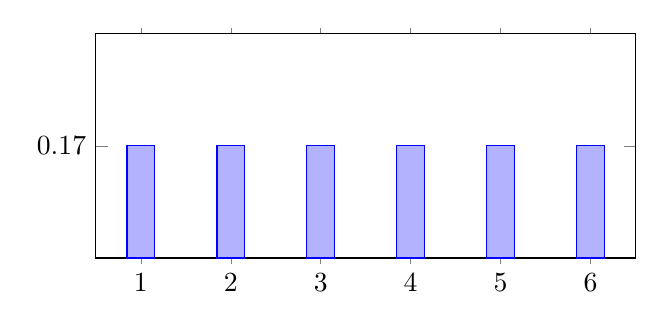
\begin{tikzpicture}
	\begin{axis}[ybar,ytick=data, anchor=north, yscale=.5]
	\addplot
	coordinates {
		(1, 1/6)
		(2, 1/6)
		(3, 1/6)
		(4, 1/6)
		(5, 1/6)
		(6, 1/6)};
	\end{axis}
	\end{tikzpicture}
	\end{center}
	\label{fig:pbDobbelsteen}
	\caption{De kansverdeling in grafiek voor het smijten van een dobbelsteen.}
\end{figure}

Een ander voorbeeld is het gooien van twee dobbelstenen met de mogelijke uitkomst. Je hebt volgens de productregel $6 \times 6 = 36$ mogelijke uitkomsten. Om bijvoorbeeld drie te gooien heb je twee mogelijkheden (kans $P(X=3) = \frac{2}{36}$). Zie voor de andere getallen tot en met 7 de tabel ($ P[X=n] = \frac{n-1}{36}$).

Als we dit nu in een histogram (zie figuur \ref{fig:pbTweedobbelstenen}) steken bekomen we een mooie trap naar boven tot 7 en dan weer naar beneden. Nu kan je makkelijk zien dat:
\begin{itemize}
  \item Voor de kans om 10 of meer te gooien moet je bijvoorbeeld die blauwe oppervlakte hebben.
  \item Voor de kans op een aantal meer dan 2 maar minder dan 7 moet je de rode oppervlakte hebben.
  \item Voor de kans op een aantal meer dan 7 maar minder dan 10 moet je de groene oppervlakte hebben.
  \item Dan is het ook logisch dat de totale oppervlakte 1 is: de kans dat 1 van al die mogelijkheden voorkomt is natuurlijk 100\%.
\end{itemize}
\begin{figure}
    \begin{center}
	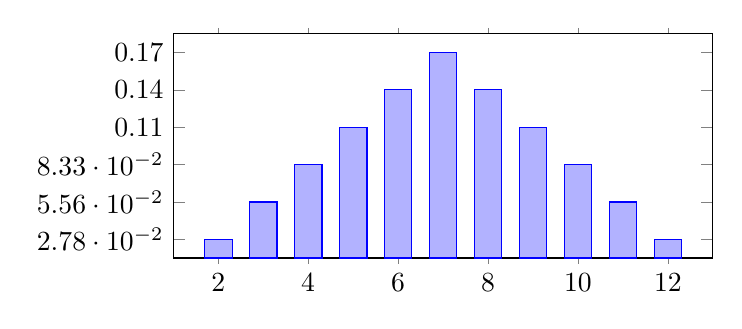
\begin{tikzpicture}
	\begin{axis}[ybar,ytick=data, anchor=north, yscale=.5]
	\addplot
	coordinates {
		(2, 1/36)
		(3, 2/36)
		(4, 3/36)
		(5, 4/36)
		(6, 5/36)
		(7, 6/36)
		(8, 5/36)
		(9, 4/36)
		(10, 3/36)
		(11, 2/36)
		(12, 1/36)
	};
	
	\end{axis}
	\end{tikzpicture}
\end{center}
	\label{fig:pbTweedobbelstenen}
	\caption{Kansverdeling voor het smijten van twee dobbelstenen.}
\end{figure}

\subsubsection{Continue kansverdeling}

Continue kansverdelingen zijn verdelingen waarbij hetgeen we meten niet alleen een beperkt aantal waarden kan aannemen (nominaal en ordinaal meetniveau), maar ook alle er tussenliggende waarden (ratio- en intervalniveau). Neem bijvoorbeeld het gewicht van onze superhelden. Dat is continu, immers dat kan niet alleen $60$ of $70$ kilo zijn, maar ook (bij benadering)  $66,8735485653$ kilo. In principe zijn alle tussenliggende waarden mogelijk (al is dat in praktijk vaak niet te meten). Dat heeft een belangrijk gevolg voor de kansverdeling. Die bestaat nu (in theorie) niet meer uit losse staafjes, maar is een vloeiende kromme geworden. Dat betekent dat de kans op bijvoorbeeld precies $70$ kilogram een kans nul heeft. Bij precies $70$ kg hoort een verticaal lijntje, en een lijntje heeft oppervlakte nul. Nu is die kans natuurlijk ook nul. Als we zeggen $70$ kg, dan bedoelen we meestal tussen $69,5$ en $70,5$, of preciezer het interval $[69,5; 70,5[$. Als we zeggen $70,00000$ kg, dan bedoelen we iets als binnen $[70,000005; 69,999995[$ kg.

De twee regels voor kansverdelingen hierboven blijven gewoon geldig. Als zo'n kromme een goede kansverdeling is, dan moet de totale oppervlakte ervan 1 zijn, en dan kun je de kans op een gewicht dat bijvoorbeeld tussen de 60 en 70 kg ligt uitrekenen door de oppervlakte hiernaast te bepalen (merk op dat het uiteindelijk niet belangrijk is of die $60$ en $70$ zelf ook nog tot het interval behoren, die hebben toch kans nul!).

\section{De normale verdeling}
\label{sec:normale-verdeling}

\begin{figure}[t]
\centering
\begin{tikzpicture}
\begin{axis}[
  domain=0:10, samples=100,
  axis lines*=left, xlabel=$x$, ylabel=$y$,
  every axis y label/.style={at=(current axis.above origin),anchor=south},
  every axis x label/.style={at=(current axis.right of origin),anchor=west},
  height=5cm, width=12cm,
  xtick={5,3.5,6.5}, ytick=\empty,
  enlargelimits=false, clip=false, axis on top,
  grid = major
  ]
  \addplot [fill=cyan!20, draw=none, domain=0:9] {gauss(5,1.5)} \closedcycle;
  \draw [yshift=-0.6cm, latex-latex](axis cs:3.5,0) -- node [fill=white] {$\sigma$} (axis cs:5.0,0);
\end{axis}
\end{tikzpicture}
\caption{De kansverdeling van de reactiesnelheid van superman. Deze grafiek noemen we de normaalverdeling met gemiddelde $\mu = 5$ ms en standaarddeviatie $\sigma = 1,5 ms.$}
\label{fig:verdelingReactievermogen}
\end{figure}


In figuur \ref{fig:verdelingReactievermogen} tonen we de kansverdeling van de reactiesnelheid X van superman. Deze grafiek noemen we de normaalverdeling met gemiddelde 5 ms en standaarddeviatie 1,5 ms. Symbolisch:
\[ X  \sim Nor(\mu = 5; \sigma = 1,5) \]

De functie die hiermee gepaard gaat is de volgende:

\begin{equation}
  f(x) = \frac{1}{\sigma \sqrt{2\pi}} e^{-\frac{1}{2} \frac{(x - \mu)^{2}}{\sigma^{2}}}
  \label{eq:normalFunction}
\end{equation}

De normale verdeling kent volgende eigenschappen:
\begin{itemize}
  \item Normale verdeling is klokvormig
  \item De normale verdeling is symmetrisch
  \item Vanwege symmetrie is gemiddelde, mediaan en modus aan elkaar gelijk
  \item De totale oppervlakte onder de klokvormige figuur is 1
  \item In gebied $\sigma$ onder $\mu$ en $\sigma$ boven $\mu$ (het zogenoemde sigma gebied) ligt ongeveer 68\% van de waarnemingen.
  \item In het gebied $2\sigma$ boven en onder $\mu$ ligt ongeveer 95\% van alle waarnemingen.
  \item Voor de verschillende gebieden zie figuur \ref{fig:standaardNormaleVerdeling}
\end{itemize}

\subsection{De standaardnormale verdeling}

Indien de toevalsveranderlijke $X \sim N(\mu,\sigma)$ verdeeld is dan is de toevalsvariabele $Z = \frac{X - \mu}{\sigma}$ normaal verdeeld: $Z \sim N(0,1)$. Dit noemen we de standaardnormale verdeling.

  % Bron: http://johncanning.net/wp/?p=1202
  \begin{center}
  \begin{figure}
  \centering
    \begin{tikzpicture}
      \begin{axis}[
          no markers, domain=0:10, samples=100,
          axis lines*=left,height=6cm, width=10cm,
          xtick={-3, -2, -1, 0, 1, 2, 3}, ytick=\empty,
          enlargelimits=false, clip=false, axis on top,
          grid = major
        ]
        \addplot [smooth,fill=cyan!20, draw=none, domain=-3:3] {gauss(0,1)} \closedcycle;
        \addplot [smooth,fill=orange!20, draw=none, domain=-3:-2] {gauss(0,1)} \closedcycle;
        \addplot [smooth,fill=orange!20, draw=none, domain=2:3] {gauss(0,1)} \closedcycle;
        \addplot [smooth,fill=blue!20, draw=none, domain=-2:-1] {gauss(0,1)} \closedcycle;
        \addplot [smooth,fill=blue!20, draw=none, domain=1:2] {gauss(0,1)} \closedcycle;
        \addplot[<->] coordinates {(-1,0.4) (1,0.4)};
        \addplot[<->] coordinates {(-2,0.3) (2,0.3)};
        \addplot[<->] coordinates {(-3,0.2) (3,0.2)};
        \node[coordinate, pin={68.3\%}] at (axis cs: 0, 0.35){};
        \node[coordinate, pin={95.4\%}] at (axis cs: 0, 0.25){};
        \node[coordinate, pin={99.7\%}] at (axis cs: 0, 0.15){};
        \node[coordinate, pin={34.1\%}] at (axis cs: -0.5, 0){};
        \node[coordinate, pin={34.1\%}] at (axis cs: 0.5, 0){};
        \node[coordinate, pin={13.6\%}] at (axis cs: 1.5, 0){};
        \node[coordinate, pin={13.6\%}] at (axis cs: -1.5, 0){};
        \node[coordinate, pin={2.1\%}] at (axis cs: 2.5, 0){};
        \node[coordinate, pin={2.1\%}] at (axis cs: -2.5, 0){};
      \end{axis}
    \end{tikzpicture}
    \caption{De standaardnormale verdeling met opdeling in zones}
    \label{fig:standaardNormaleVerdeling}
    \end{figure}
  \end{center}

In het algemeen kan men dus bij een waarneming $x$ de zogenaamde $z$-score bepalen als volgt:

\begin{equation}
  z = \frac{x-\mu}{\sigma}
  \label{eq:zscore}
\end{equation}

Deze score geeft dus aan hoe extreem een waarneming is of anders gezegd, hoeveel standaarddeviaties is de waarneming $x$ van het gemiddelde $\mu$ verwijderd. Voor een willekeurige $x$-waarde kunnen we met formule \ref{eq:zscore} de bijhorende $z$-score bepalen. Voor deze $z$-scores heeft men tabellen opgesteld met de kansen dat een waarde kleiner dan $z$ getrokken wordt uit Z, de zgn.~linkerstaartkans\footnote{Er bestaan ook tabellen met de rechterstaartkans}: $P(Z<z)$.

R heeft eveneens functies voor het rekenen met kansen van normaal verdeelde variabelen. Deze worden samengevat in Tabel~\ref{rab:norm-prob-r}.

\begin{table}
  \centering
  \begin{tabular}{ll}
  	\textbf{Functie}      & \textbf{Betekenis}                                             \\ \hline
  	\verb|pnorm(x, m, s)| & Linkerstaartkans, $P(X<\mathtt{x})$                            \\
  	\verb|dnorm(x, m, s)| & Hoogte van de Gausscurve op punt \texttt{x}                    \\
  	\verb|qnorm(p, m, s)| & Onder welke grens zal \texttt{p}\% van de waarnemingen liggen? \\
  	\verb|rnorm(n, m, s)| & Genereer \texttt{n} normaal verdeelde random getallen
  \end{tabular}

  \caption{Kansberekeningsfuncties in R voor een normale verdeling met gemiddelde \texttt{m} en standaardafwijking \texttt{s}. Indien argumenten \texttt{m} en \texttt{s} weglaten worden, wordt de standaardnormaalverdeling verondersteld.}
  \label{rab:norm-prob-r}
\end{table}

We komen dan tot de volgende methode voor het berekenen van kansen met de normale verdeling:
\begin{enumerate}
  \item Bepaal de kansvariabele met de bijbehorende normale verdeling
  \item Bereken de $z$-score bij de bijhorende $x$-waarde.
  \item Schets de plaats van de gevraagde kans
  \item Herleid de gevraagde kans met behulp van de schets tot een linkerstaartkans en gebruik de $z$-tabel van de standaardnormale verdeling om deze te bepalen. Gebruik indien nodig de symmetrieregel en de regel van 100\% kans.
\end{enumerate}

\begin{example}
Hoe groot is de kans dat superman in minder dan 4 ms reageert?
\[ P(X < 4) = P(Z < -0,67) = 0,2514 \]
\end{example}
\begin{example}
Hoe groot is de kans dat hij in minder dan 7 ms reageert?
\[ P(X < 7) = P(Z < 1,33) = 0,9082 \]
\end{example}
\begin{example}
Hoe groot is de kans dat superman in minder dan 3 ms reageert?
\[ P(X<3) = P(Z < -1,33) = 0,0918 \]
\end{example}
\begin{example}
Hoe groot is de kans dat hij reageert tussen de 2 en 6,5 ms
\[ P( 2 < X < 6,5) = P(X<6,5) - P(X<2) = P(Z<1) - P(Z<-2) = 0,8186 \]
\end{example}

\subsection{Testen op normaliteit}
\label{sec:normtesting}

Er zijn verschillende methoden die kunnen gebruikt worden om na te gaan of een steekproef uit een normale verdeling komt.
\begin{enumerate}
  \item Construeer een histogram voor de gegevens en bekijk de vorm van de grafiek. Als de gegevens bij benadering een normale verdeling hebben, zal de vorm van het histogram een klokcurve vormen.
  \item Bereken de intervallen $\overline{x} \pm s$, $\overline{x} \pm 2s$, $\overline{x} \pm 3s$ en bepaal het percentage meetwaarden dat binnen elk van deze intervallen valt. Als de gegevens ongeveer normaal verdeeld zijn, zullen de percentages ongeveer gelijk zijn aan respectievelijk 68\%, 95\% en 99,7\%.
  \item Construeer een QQ-plot (normaliteitsplot, zie Definitie~\ref{def:qq-plot}) voor de gegevens. Als de gegevens ongeveer normaal verdeeld zijn, zullen de punten ongeveer op een rechte lijn liggen.
  \item Bereken de \emph{kurtosis} (``welving'' of ``platheid''): duidt aan hoe scherp de ``piek'' van de verdeling is.
    \begin{itemize}
      \item Een normale verdeling heeft een kurtosis = 0
      \item Een vlakke distributie heeft een negatieve kurtosis
      \item Een eerder piekvormige distributie heeft een positieve kurtosis
      \item Let op: bij de originele definitie van kurtosis (zoek die eens op!) heeft de normale verdeling een kurtosis van 3. Wij gebruiken hier een alternatieve definitie, meestal de ``excess kurtosis'' genoemd, waar men 3 aftrekt van de originele waarde, zodat je op 0 uitkomt.
    \end{itemize}
  \item Bereken de \emph{Skewness} (scheefheid): duidt aan hoe symmetrisch de data is.
    \begin{itemize}
      \item Een symmetrische distributie heeft een skewness = 0
      \item Bijgevolg: een normale verdeling heeft een skewness = 0.
      \item Een distributie met een lange linkerstaart heeft een negatieve skewness
      \item Een distributie met een lange rechterstaart heeft een positieve skewness
      \item Vuistregel: absolute waarde van skewness $>1$, geen symmetrische distributie.
    \end{itemize}
\end{enumerate}

\begin{definition}[QQ-plot of normaliteitsplot]
  \label{def:qq-plot}
  Een normaliteitsplot of QQ-plot\footnote{Q staat hier voor \emph{quantile}, kwantiel} voor een gegevens\-verzameling is een spreidingsdiagram met de gesorteerde gegevenswaarden op de ene as en de bijbehorende verwachte $z$-waarden van een standaardnormale verdeling op de andere as. Zie figuur~\ref{fig:qqplot} voor enkele voorbeelden. De R-code voor het genereren van deze afbeeldingen is hieronder gegeven.
\end{definition}

\begin{figure}
  \begin{center}
    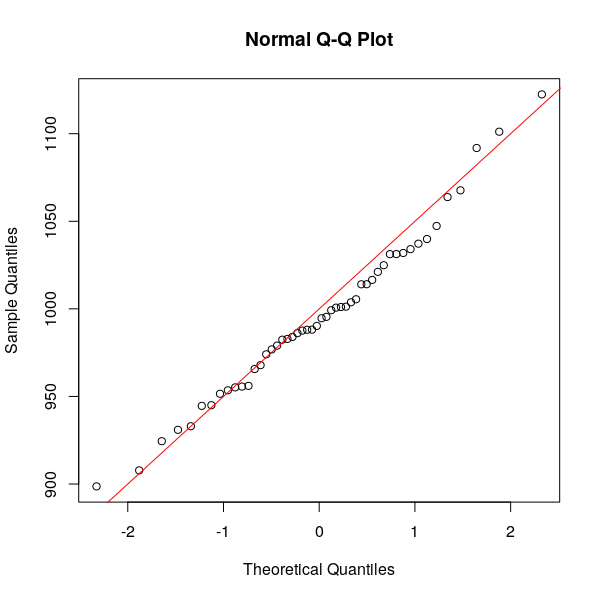
\includegraphics[width=.45\textwidth]{sampling-qqplot-good}
    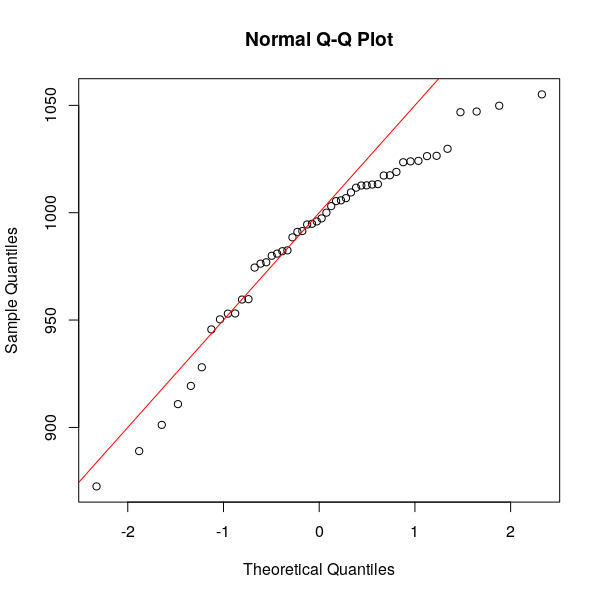
\includegraphics[width=.45\textwidth]{sampling-qqplot-bad}
  \end{center}
  \caption{De QQ-plot links is gebaseerd op een steekproef van 50 observaties uit een normale distributie met gemiddelde 1000 en standaardafwijking 50. De rechterplot is gebaseerd op een Student-$t$ distributie met 15 vrijheidsgraden. Het aantal observaties, gemiddelde en standaardafwijking zijn hetzelfde als links.
    De lijnen in het rood duiden aan waar zich in theorie de observaties zouden moeten bevinden. Links is dat min of meer zo, maar rechts wijken de observaties af, vooral in de extremen.}
  \label{fig:qqplot}
\end{figure}

\lstinputlisting{data/qqplot.R}

\section{Centrale limietstelling}
\label{sec:centrale-limietstelling}

\begin{definition}[Lineaire combinatie van onafhankelijke, gelijk verdeelde stochasten]
Formeel: Een lineaire combinatie van onafhankelijke, gelijk verdeelde stochasten is steeds normaal verdeeld.

\[X_{i} \sim Nor(\mu_{i}, \sigma_{i}) \Rightarrow Y = \sum_{i} \alpha_{i} X_{i} \textnormal{ ook normaal verdeeld} \]

Bijgevolg zal ook het steekproefgemiddelde van een steekproef uit een populatie met een willekeurige verdeling, nagenoeg normaal verdeeld zijn voor een voldoende grote $n$.
\end{definition}

Wanneer men dus een aselecte steekproef neemt van onafhankelijke variabelen met een normale verdeling, dan zegt de centrale limietstelling dat het gemiddelde van deze steekproef bij benadering normaal verdeeld zal zijn. Dus als men steeds opnieuw een steekproef neemt met dezelfde grootte, en telkens het gemiddelde optekent, bekomt men bij benadering de grafiek van een normale verdeling. Hoe groter de steekproef, hoe beter de benadering. Het steekproefgemiddelde is dus normaal verdeeld, onafhankelijk van de onderliggende verdeling van de grootheid waarvan men een steekproef neemt. Algemeen kunnen we volgende stelling poneren:

\begin{definition}[Centrale limietstelling]
Beschouw een aselecte steekproef van $n$ waarnemingen die uit een populatie met verwachtingswaarde $\mu$ en standaardafwijking $\sigma$ wordt genomen. Als $n$ groot genoeg is zal de kansverdeling van het steekproefgemiddelde $\overline{x}$ een normale verdeling benaderen met verwachting $\mu_{\overline{x}} = \mu$ en standaardafwijking $\sigma_{\overline{x}} = \frac{\sigma}{\sqrt{n}}$. Hoe groter de steekproef is, des te beter zal de kansverdeling van $\overline{x}$ de verwachtingswaarde van de populatie benaderen.

\end{definition}

Bij het afnemen van een steekproef is zelden de onderliggende verdeling gekend, en toch kan men uitspraken doen over de gemiddelde waarde. Dit is volledig te danken aan de centrale limietstelling, die dit gemiddelde een regel oplegt los van de onderliggende kansverdeling. De centrale limietstelling houdt het steekproefgemiddelde in bedwang, sluit het op in de Gaussische kooi waaruit het nooit kan ontsnappen. Dit, en alleen dit, laat wetenschappers toe het nauwkeurig te bestuderen, te observeren en stelt hen in staat te concluderen.

Want, mocht de verdeling van het steekproefgemiddelde afhankelijk zijn van de onderliggende verdeling, een resultaat dat men tot op zekere hoogte zelfs zou verwachten, zou het onmogelijk zijn om concrete uitspraken te doen over vele wetenschappelijke resultaten. In de theoretische statistiek duiken vrijwel constant limieten van steekproefgemiddeldes op, en deze kunnen dankzij de centrale limietstelling zonder verpinken vervangen worden door een normale verdeling. Zou dit niet mogelijk zijn, dan zou de ganse theorie rond het schatten van parameters in elkaar storten wat dan weer rampzalig zou zijn voor de praktijk. Onderzoeken vergelijken zou herleid worden tot een quasi onmogelijke opgave, en de statistiek in het algemeen zou veel lastiger en ingewikkelder worden.

\subsection{Toepassing van de centrale limietstelling}
Bij het trekken van een aselecte steekproef van omvang $n$ uit een populatie met (onbekend) gemiddelde $\mu$ en standaarddeviatie $\sigma$ is de kansverdeling van het steekproefgemiddelde een kansvariabele $M \sim N (\overline{x}, \frac{\sigma}{\sqrt{n}})$, op voorwaarde dat de steekproefomvang voldoende groot is.

\begin{example}
  We bekijken nu de reactiesnelheid van al onze superhelden en uit onze steekproef met $n = 100$ en $\overline{x} = 90, \sigma = 60$ (miliseconden). Dan kunnen we ons de vraag stellen: wat is de kans dat de gemiddelde reactiesnelheid van een superheld minder is dan $104$ ms?


  \begin{enumerate}
    \item De kansvariabele hier is de gemiddelde reactiesnelheid $\overline{x}$ in een steekproef van $n=100$ superhelden. Daarom geldt wegens de centrale limietstelling:
    \[ \overline{x} \sim Nor(\mu = 90, \sigma_{\overline{x}} = \frac{60}{\sqrt{100}} = 6) \]
    \item We kunnen hierbij de passende $z$-score bepalen:
    \[ z = \frac{104-90}{\frac{60}{\sqrt{100}}} = \frac{104-90}{6} = 2,33 \]
    Dus geldt : $P(\overline{x} < 104) = P(Z < 2,33) = 1 - 0,0099 \approx 0,99$
  \end{enumerate}
\end{example}

\subsection{Schatten van een parameter}

Indien we nu een steekproef onderzoeken, willen we uit de berekening op de steekproef een aantal conclusies kunnen trekken met betrekking tot de populatie. We willen bijvoorbeeld de gemiddelde kracht kennen van een superheld of de fractie superhelden die rijk zijn. Als we een schatting geven voor dergelijke onbekende parameter, noemen we dat ook een puntschatter. We gebruiken bijvoorbeeld $\overline{x}$ als schatter om $\mu$ te schatten.

\begin{definition}[puntschatter]
  Een puntschatter voor een populatieparameter is een regel of een formule die ons zegt hoe we uit de steekproef een getal moeten berekenen om de populatieparameter te schatten.
\end{definition}

\subsection{Betrouwbaarheidsinterval populatiegemiddelde bij grote steekproef}
\label{ssec:betrouwbaarheidsinterval-grote-steekproef}

In het geval het schatten van een gemiddelde van een populatie uit een steekproef hebben we totaal geen idee over hoe correct onze schatting is. Daarvoor gaan we op zoek naar een interval waarvan we met een bepaalde zekerheid, bv. 95\%, kunnen zeggen dat het de te schatten karakteristiek bevat.

\begin{definition}[Betrouwbaarheidsinterval]
Een betrouwbaarheidsinterval is een regel of een formule die ons zegt hoe we uit de steekproef een interval moeten berekenen dat de waarde van de parameter met een bepaalde hoge waarschijnlijkheid bevat.
\end{definition}

Een eerste goede schatting voor populatiegemiddelde zou het steekproefgemiddelde zijn:

\[ \overline{x} = \frac{1}{n} \sum_{i} x_{i} \]

Natuurlijk is deze schatting niet de werkelijke waarde van de populatie. Daarom wordt vaak rondom $\overline{x}$ een interval geconstrueerd dat de waarden bevat die aannemelijk zijn voor $\mu$. Hiervoor kunnen we gebruik maken van de centrale limietstelling: het gemiddelde in een te trekken steekproef van omvang $n$ is normaal verdeeld met karakteristieken $\mu$ en $\frac{\sigma}{\sqrt{n}}$.  Als we nu het gemiddelde standaardiseren krijgen we:

\[ Z = \frac{\overline{x} - \mu}{\frac{\sigma}{\sqrt{n}}} \]

Deze uitdrukking hangt van $\mu$ af maar we weten wel dat deze standaardnormaal verdeeld is. We kunnen daarom getallen $-z$ en $z$ vinden, onafhankelijk van $\mu$, waartussen $Z$ met een gekozen kans $1 - \alpha$ ligt. Deze kans $1 - \alpha$ wordt het \emph{betrouwbaarheidsniveau}\index{betrouwbaarheidsniveau}\index{niveau!betrouwbaarheids-} genoemd. We nemen hier $1 - \alpha= 0,95$.

\[P(-z < Z < z) = 1 - \alpha = 0,95 \]

Hieruit halen we dat $\alpha = 0,05$. Door het toepassen van de symmetrieregel weten we dus dat we volgende term moeten berekenen:

\[ P( Z < z) = 1 - 0,025 \]

Kijken we in de Z-tabel dan vinden we voor de rechterstaartkans $0,025$ de z-score van $1,96$.

Dus vinden we :

\[ P( -1,96 < \frac{\overline{x} - \mu}{\frac{\sigma}{\sqrt{n}}} < 1,96 ) \]
en dus
\[ P ( \overline{x} -1,96 \frac{\sigma}{\sqrt{n}} <\mu < \overline{x} + 1,96 \frac{\sigma}{\sqrt{n}}) \]

Op die manier kunnen we dus grenzen bepalen die een interval aanduidt waar 95\% kans is dat $\mu$ gevonden wordt. Formeel: als je herhaalde steekproeven zou nemen en telkens op basis van het gerealiseerde steekproefgemiddelde $\overline{x}$ een betrouwbaarheidsinterval zou maken, dan zal bij 95\% van de intervallen $\mu$ binnen de intervalgrenzen liggen.

Opgelet, we gaan er hier van uit dat we de standaarddeviatie van de populatie kennen, wat meestal niet zo is. Indien de steekproef groot genoeg is, kunnen we de steekproefstandaarddeviatie nemen als schatter voor de standaarddeviatie voor de populatie.

\[ P ( \overline{x} -1,96 \frac{\sigma_{\overline{x}}}{\sqrt{n}} < \mu < \overline{x} + 1,96 \frac{\sigma_{\overline{x}}}{\sqrt{n}}) \]


\begin{figure}[t]
\centering
\begin{tikzpicture}
\begin{axis}[
  domain=-3:3, samples=100,
  axis lines*=left, xlabel=$z$,
  every axis y label/.style={at=(current axis.above origin),anchor=south},
  every axis x label/.style={at=(current axis.right of origin),anchor=west},
  height=5cm, width=12cm,
  xtick={-1.96,0,1.96}, ytick=\empty,
  enlargelimits=false, clip=false, axis on top,
  grid = major
  ]
  \addplot [fill=cyan!20, draw=none, domain=-3:3] {gauss(0,1)} \closedcycle;
  \draw [yshift=-0.6cm, latex-latex](axis cs:-1.96,0) -- node [fill=white] {$\sigma$} (axis cs:1.96,0);
\end{axis}
\end{tikzpicture}
\caption{Standaardnormale verdeling die 95\% betrouwbaarheidsinterval aanduidt.}
\label{fig:verdelingStandaardnormaal}
\end{figure}

\subsection{Betrouwbaarheidsinterval populatiegemiddelde bij een kleine steekproef}
\label{ssec:betrouwbaarheidsinterval-kleine-steekproef}

Bij kleine steekproeven kunnen we niet langer veronderstellen dat de kansverdeling van $\overline{x}$ bij benadering
normaal verdeel is, omdat de centrale limietstelling alleen normaliteit garandeert voor grote steekproeven ($n >30$). De vorm
van de kansverdeling van het steekproefgemiddelde $\overline{x}$ hangt nu af van de vorm van de verdeling van de populatie waaruit de
steekproef genomen wordt. Alhoewel nog steeds geldt dat $\sigma_{\overline{x}} = \frac{\sigma}{\sqrt{n}}$ kan
de standaardafwijking $s$ een slechte benadering zijn voor $\sigma$ als de steekproef klein is.

Als oplossing kunnen we een nieuwe grootheid bepalen. In plaats van

\[ z = \frac{\overline{x} - \mu}{\frac{\sigma}{\sqrt{n}}} \]

construeren we

\[ t = \frac{\overline{x} - \mu}{\frac{s}{\sqrt{n}}} \]

Deze heeft een kansverdeling die beschreven wordt door een Student-t verdeling. Deze lijkt zeer goed op de normale verdeling: klokvormig, symmetrisch en met verwachtingswaarde 0.

De precieze vorm van de kansverdeling $t$ hang af van de steekproefomvang $n$. We zeggen dat de t-verdeling $(n-1)$ vrijheidsgraden heeft (afgekort $df$).
Merk op dat:
\begin{itemize}
  \item $(n-1)$ ook gebruikt werd om $s^{2}$ te berekenen
  \item als $n \rightarrow \infty$ we de standaardnormale verdeling verkrijgen.
\end{itemize}

Indien we nu een betrouwbaarheidsinterval willen bepalen voor een steekproef met een klein aantal waarden moeten we het volgende doen:

\begin{definition}[Betrouwbaarheidsinterval kleine steekproef]
  Om een betrouwbaarheidsinterval voor het gemiddelde te bepalen op basis van een klein steekproef bepalen we:
  \[ \overline{x} \pm t_{\frac{\alpha}{2}}(\frac{s}{\sqrt{n}}) \]
  waarbij $t_{\frac{\alpha}{2}}$ gebaseerd is op $(n-1)$ vrijheidsgraden. We veronderstellen wel dat we een aselecte steekproef genomen hebben uit
  een populatie die bij benadering normaal verdeeld is.
\end{definition}

\begin{table}
  \centering
  \begin{tabular}{ll}
  	\textbf{Functie} & \textbf{Betekenis}                                             \\ \midrule
  	\verb|pt(x, df)| & Linkerstaartkans, $P(X<\mathtt{x})$                            \\
  	\verb|dt(x, df)| & Hoogte van de curve op punt \texttt{x}                         \\
  	\verb|qt(p, df)| & Onder welke grens zal \texttt{p}\% van de waarnemingen liggen? \\
  	\verb|rt(n, df)| & Genereer \texttt{n} random getallen volgens deze verdeling
  \end{tabular}

  \caption{Kansberekeningsfuncties in R voor de Student-$t$ verdeling met \texttt{df} vrijheidsgraden, verwachte waarde 0 en standaardafwijking 1.}
  \label{tab:t-prob-r}
\end{table}

\subsection{Betrouwbaarheidsinterval voor populatiefractie bij een grote steekproef}
\label{ssec:betrouwbaarheidsinterval-populatiefractie}

Indien je een variabele wil meten als een fractie, bijvoorbeeld \% mensen die ja geantwoord heeft op een bepaalde vraag, dan willen we in feite de kans $p$ op succes in een bernouilli experiment schatten, waarbij $p$ de kans is dat een willekeurig geselecteerde respondent (of element van de populatie) een succes is (succes in termen van binomiaal experiment). We kunnen $p$ dan schatten door bijvoorbeeld:

\[ \overline{p} = \frac{\textnormal{aantal successen}}{n} \]

Om nu de betrouwbaarheid van de schatter $\overline{p}$ te bepalen moeten we de kansverdeling kennen van $\overline{p}$. Dit kunnen we beredeneren door toepassing van de centrale limietstelling op het gemiddelde aantal successen in de steekproef van omvang $n$. Indien succes = 1 en faling = 0, dan hebben we een steekproef van $n$ elementen, ieder met dezelfde verdeling (kans op 1 is $p$ en kans op 0 is $q=1-p$).  Het gemiddelde $\overline{p}$ heeft dan bij benadering een normale verdeling. Of dus:

\begin{itemize}
  \item Verwachting van kansverdeling van $\overline{p}$ is $p$.
  \item De standaardafwijking van kansverdeling $\overline{p} = \sqrt{\frac{pq}{n}}$
  \item Voor grote steekproeven is $\overline{p}$ bij benadering normaal verdeeld.
\end{itemize}

Aangezien $\overline{p}$ een steekproefgemiddelde is van het aantal successen, stelt dit ons in staat een betrouwbaarheidsinterval te berekenen analoog als die voor de intervalschatting van $\mu$ voor grote steekproeven.

\begin{definition}[Betrouwbaarheidsinterval voor $p$ gebaseerd op grote steekproef]
  \[ \overline{p} \pm z_{\frac{\alpha}{2}} \sqrt{\frac{\overline{p}\overline{q}}{n}} \]
  met $\overline{p} = \frac{x}{n}$ en $\overline{q} = 1- \overline{p}$
\end{definition}


\section{R}
We kijken naar enkele basisoperaties die verband houden met enkele distributies. Er zijn een groot aantal verdelingen beschikbaar, maar we kijken maar naar een paar. Als u wilt weten welke distributies beschikbaar zijn, kunt u een zoekopdracht uitvoeren met behulp van de opdracht

\begin{lstlisting}
> help.search ("distribution").
\end{lstlisting}


Hier geven we details over de commando's die verband houden met de normale distributie en vermelden kort de commando's voor andere distributies. De functies voor verschillende verdelingen zijn zeer vergelijkbaar.

De prefixen zijn als volgt:
\begin{description}
	\item[d] geeft de hoogte van de respectievelijke kansdichtheidsfunctie
	\item[p] geeft de cumulatieve kansdichtheidsfunctie
	\item[q] geeft de omgekeerde cumulatieve dichtheidsfunctie
	\item[r] geeft een willekeurige waarde
\end{description}

\subsection{De normale verdeling}
Er zijn vier functies die kunnen worden gebruikt om de waarden geassocieerd met de normale distributie te genereren.
\subsubsection{dnorm}

De eerste functie waarnaar we kijken, is \texttt{dnorm}. Gegeven een waarde geeft het de hoogte van de kansverdeling op elk punt terug. Als u alleen de punten zonder gemiddelde en standaardafwijking ingeeft wordt een gemiddelde van nul en standaardafwijking van 1 beschouwd. Er zijn opties om verschillende waarden voor de gemiddelde en standaardafwijking te gebruiken.

\lstinputlisting{data/norm.R}

\subsubsection{pnorm}

Dit is de cumulatieve kansdichtheidsfunctie, of anders gezegd de linkerstaartkans: \texttt{pnorm(x)} is $P(Z < x)$.

\subsubsection{qnorm}
De volgende functie die we bekijken is \texttt{qnorm}, die de inverse van \texttt{pnorm} is. Het idee achter \texttt{qnorm} is dat je het een kans $\alpha$ geeft, en het geeft het getal weer waarvan de cumulatieve distributie overeenkomt met de waarschijnlijkheid $\alpha$.

\lstinputlisting{data/qnorm.R}

\subsubsection{rnorm}

De laatste functie die we onderzoeken is de \texttt{rnorm} functie die willekeurige getallen kan genereren waarvan de distributie normaal is. Het argument dat je ingeeft is het aantal willekeurige getallen dat u wilt, met optionele argumenten om de gemiddelde en standaardafwijking op te geven:

\lstinputlisting{data/rnorm.R}

\section{Oefeningen}
\label{sec:steekproefonderzoek-oefeningen}

\begin{exercise}
  \label{ex:prob-norm-dist}
  Bereken ook elke keer het gevraagde gebied.
  \begin{enumerate}[label=\alph*.]
    \item $P(Z < 1.33)$
    \item $P(Z > 1.33)$
    \item $P(Z < -1.33)$
    \item $P(Z > -1.33)$
    \item $P(Z < 0.45)$
    \item $P(Z > -1.05)$
    \item $P(Z < 0.65)$
    \item $P(-0.45 < Z < 1.20)$
    \item $P(-1.35 < Z < -0.10)$
    \item $P(-2.10 < Z < -0.90)$
  \end{enumerate}
\end{exercise}

\begin{exercise}
	Bepaal de dichtheid en de cumulatieve waarschijnlijkheidscurve voor een normale verdeling met een gemiddelde $\mu$
	van 2,5 en $\sigma = 1,5$. Bepaal de oppervlakte voor het gebied onder de dichtheidscurve tussen
	$x = 0.5$ en $x = 4$. Controleer uw antwoord door de berekening te doen.
\end{exercise}

\begin{exercise}
	Bepaal de dichtheid en de cumulatieve waarschijnlijkheidscurve voor een t-verdeling met $df = 3$. Teken ook een normale verdeling met een $\mu = 0$  en $\sigma = 1$.
\end{exercise}

\begin{exercise}
Gebruik de functie \verb|rnorm()| een willekeurige steekproef van 25 waarden uit een normale verdeling te tekenen met een gemiddelde van 0 en een standaardafwijking gelijk aan 1,0. Gebruik een histogram, met \verb|probability = TRUE|.

Maak een overlay over het histogram met: (a) de theoretische dichtheidscurve voor een normale verdeling met gemiddelde 0 en standaardafwijking gelijk aan 1,0; (b) een ``geschatte'' dichtheidscurve op basis van het gemeten steekproefgemiddelde en -standaardafwijking.

Herhaal dit voor een steekproef van 100 en 500 waarden.
\end{exercise}

\begin{exercise}
  In de  Hogeschool zijn er twee klassen voor het vak onderzoekstechnieken. De studenten werden willekeurig over de klassen verdeeld, zodat we mogen veronderstellen dat de ene klas niet slimmer is dan de andere. In de A-klas geeft mevr. X les, in de B-klas geeft mr. Y les. X is nogal streng en op het einde van het schooljaar behaalt haar klas een gemiddelde van 54 op 100 met een standaardafwijking van 11.

  Y is iets losser en stimuleert de leerlingen al gauw met een puntje meer. Op het einde van het schooljaar behaalt zijn klas een gemiddelde van 62 op 100 en een standaardafwijking van 7.

  Wouter zit in de A-klas en heeft $\frac{63}{100}$ voor wiskunde. Stijn zit in de B-klas en behaalt $\frac{67}{100}$. Wie heeft volgens jou het beste gescoord binnen de eigen klas?
\end{exercise}

\begin{exercise}
  Een gezondheidsonderzoek tussen 1988 en 1994 gaf aan dat de gemiddelde cholesterolwaarde bij vrouwen tussen 20 en 29 jaar 183 mg/dl bedroeg, met een standaardafwijking gelijk aan 36. We nemen nu een aselecte steekproef van 81 vrouwen. Los volgende vragen op:

  \begin{enumerate}[label=\alph*.]
    \item Schets de kansdichtheidsfunctie voor de populatie en de kansverdeling van het steekproefgemiddelde $\overline{x}$.
    \item Bepaald de kans dat $\overline{x}$ kleiner is dan 185.
    \item Bepaal de kans dat $\overline{x}$ tussen 175 en 185 ligt.
    \item Bepaal de kans dat $\overline{x}$ groter is dan 190.
  \end{enumerate}
\end{exercise}

\begin{exercise}
  Een aselecte steekproef van 64 stuks wordt getrokken uit een populatie met onbekende verdeling. De verwachting en de standaardafwijking van de populatie
  zijn wel gekend: $\mu = 20$ en $\sigma=16$. Los volgende vragen op:

  \begin{enumerate}[label=\alph*.]
    \item Bepaal de verwachting en standaardafwijking van het steekproefgemiddelde.
    \item Beschrijf de vorm van de verdeling van het steekproefgemiddelde. In hoeverre hangt je antwoord af van de grootte van de steekproef?
    \item Bereken de $z$ score bij $\overline{x_{1}} = 15.5$ en $\overline{x_{2}} = 23$.
    \item Bepaal kans dat $\overline{x} <16$.
    \item Bepaal kans dat $\overline{x} > 23$.
    \item Bepaal kans dat $16< \overline{x}< 22$.
  \end{enumerate}
\end{exercise}

\begin{exercise}
  Verkeersdrempels zijn bedoeld om de snelheid van automobilisten te be\"invloeden. Afhankelijk van de gewenste snelheid in een straat worden de drempels steiler of minder steil gemaakt. Drempel A is zo ontworpen dat 85 \% van de automobilisten de drempel passeert met een snelheid van minder dan 50 km per uur. In de praktijk blijkt dat de passeersnelheid bij een drempel normaal verdeeld is. Bij drempel A werd een gemiddelde passeersnelheid van 43,1 km/h gevonden met standaardafwijking 6,6 km/h.

  \begin{enumerate}[label=\alph*.]
    \item Toon aan dat 85\% van de automobilisten niet harder dan 50 km/h rijdt.
    \item Bij hoeveel van de 1200 metingen kan, op grond van eerdere ervaringen, een snelheid van meer dan 55 km/h worden verwacht?
  \end{enumerate}
\end{exercise}

\begin{exercise}
  Een conservenfabrikant krijgt de laatste tijd klachten over de netto inhoud van zijn conserven met wortelen en erwtjes, die volgens de verpakking netto 1 liter zouden moeten bevatten. Daarom laat hij een steekproef nemen waarin de netto inhoud van 40 willekeurig gekozen blikjes wordt gecontroleerd. De resultaten worden samengevat in Tabel~\ref{tab:Steekproefwaarden}.

Vraag A:
\begin{itemize}
  \item Vul de tabel aan met de cumulatieve absolute frequentie
  \item Vul de tabel aan met de relatieve frequentie
  \item Vul de tabel aan met de cumulatieve relatieve frequentie.
\end{itemize}
Vraag B:

\begin{itemize}
  \item Bereken het gemiddelde
  \item Bereken de standaardafwijking
  \item Hoeveel procent van de blikken bevatten te weinig wortelen en erwtjes.
  \item Teken een histogram van de absolute frequentie.
  \item Zijn de gegevens normaal verdeeld?  Hoe zie je dat?
\end{itemize}

\end{exercise}

  \begin{table}
  \centering
  \begin{tabular}{lr}
    \toprule
    Inhoud & $n_{i}$ \\
    \midrule
    $[970,980[$ & 3 \\
    $[980,990[$ & 5 \\
    $[990,1000[$ & 13 \\
    $[1000,1010[$ & 11 \\
    $[1010,1020[$ & 5 \\
    $[1020,1030[$ & 3 \\
    \bottomrule
  \end{tabular}
  \caption{Steekproefwaarden}
  \label{tab:Steekproefwaarden}
\end{table}

\begin{exercise}
  Betrouwbaarheidsintervallen.
  
  \begin{enumerate}
    \item Wat is de onder- en bovengrens van een betrouwbaarheidsinterval van 99\%?
    \item Een betrouwbaarheidsinterval van 99\% is breder dan een van 95\%. Waarom is dit zo?
    \item Hoe zou het betrouwbaarheidsinterval voor 100\% er uit zien?
  \end{enumerate}
  
\end{exercise}

\begin{exercise}
  \label{ex:confidence-money}
  
  Lees de dataset \texttt{money.csv} in. We veronderstellen dat de waarden uit deze steekproef normaal verdeeld zijn rond een onbekend populatiegemiddelde $\mu$, maar dat de populatiestandaardafwijking gekend is en gelijk aan $\sigma = 99$.
  
  \begin{enumerate}
    \item Bereken een 99\%-betrouwbaarheidsinterval voor het populatiegemiddelde.
    \item Bereken een 95\%-betrouwbaarheidsinterval voor het populatiegemiddelde.
    \item Stel dat $\sigma$ onbekend is. Bereken voor dat geval een 95-\% betrouwbaarheidsinterval voor het populatiegemiddelde.
    \item Stel tenslotte een 95\%-betrouwbaarheidsinterval voor het populatiegemiddelde, in de veronderstelling dat de steekproef enkel bestaat uit de eerste 25 waarden in het databestand.
  \end{enumerate}
\end{exercise}

\begin{exercise}
  Een webhostingfirma heeft een Service Level Agreement met een klant voor een gegarandeerde uptime van ``five nines'' (99,999\%).  Die wordt aan het einde van elk jaar gecontroleerd en als de minimale uptime niet gehaald wordt, moet de hostingfirma een boete betalen.

  Om de uptime te meten, voert een monitoringsysteem elke minuut een \texttt{HTTP GET /} uit en controleert het resultaat a.h.v.
  de HTTP return code. In de maand januari is er één enkele HTTP request onsuccesvol geweest.

  \begin{itemize}
    \item Als deze trend zich voortzet, wat is de kans dat de SLA niet gehaald wordt aan het einde van het jaar? Gebruik de formule voor de kansverdeling van een fractie.
    \item De gebruikte formule is eigenlijk niet geschikt in dit specifieke geval en geeft een vertekend beeld. Wat zou de reden kunnen zijn?
  \end{itemize}
\end{exercise}

\section{Antwoorden op geselecteerde oefeningen}
\label{sec:oplossingen-steekproefonderzoek}

\paragraph{Oefening \ref{ex:prob-norm-dist}}

\begin{enumerate}[label=\alph*.]
  \item $0,908$
  \item $0,092$
  \item $0,092$
  \item $0,908$
  \item $0,674$
  \item $0,853$
  \item $0,742$
  \item $0,559$
  \item $0,372$
  \item $0,166$
\end{enumerate}

\paragraph{Oefening \ref{ex:confidence-money}}

\begin{enumerate}
  \item $[481,725; 523,368]$
  \item $[486,704; 518,390]$
  \item $[486,476; 518,617]$
  \item $[485,761; 519,332]$
\end{enumerate}